\documentclass[UTF8]{article}
\usepackage{ctex}
\usepackage{ulem}
\usepackage{amssymb}
\usepackage{amsmath}
\usepackage{graphicx}
\newtheorem{thm}{定义}[section]
\newtheorem{notation}[thm]{记号}
\newtheorem{lemma}[thm]{引理}

\makeatletter
\newcommand{\rmnum}[1]{\romannumeral #1}
\newcommand{\Rmnum}[1]{\expandafter\@slowromancap\romannumeral #1@}
\makeatother

\title{构造演算(The Calculus of Constructions)\\[2ex]\begin{large}读书笔记\end{large}}
\author{许博}
\date{}

\begin{document}
\maketitle
	\section{$\lambda{\rm C}$系统}
	\noindent
	$\lambda{\rm C}$组合了第二章到第五章中介绍的系统,拥有四种可能的选择,即依赖于项/类型的项/类型。
		
		$\lambda{\rm P}$与$\lambda{\rm C}$只有一处不同,但足以扩展$\lambda{\rm P}$到$\lambda{\rm C} = \lambda{2} + \lambda{\uline{\omega}} + \lambda{\rm P}$:
		
		$(form_{\lambda{\rm P}})\ \cfrac{\Gamma\vdash A:*\ \ \ \Gamma,x:A\vdash B:s}{\Gamma\vdash\Pi x:A.B:s}$\\
		
		在这条规则中,关键点是$A:*$,为了保证类型$\Pi x:A.B$的成员(inhabitant)是项或者依赖于项的类型。但在舍弃了这个限制之后,我们就获得了我们想要的泛化:依赖于项/类型的项/类型。
		
		看起来将$A:*$替换为$A:s$,其中$s$为$*$或$\square$,就足够了,但是规则中已经出现了$s$,观察$\lambda{\uline{\omega}}$的($form$)-规则:
		
		$(form_{\lambda{\uline{\omega}}})\ \cfrac{\Gamma\vdash A:s\ \ \ \Gamma\vdash B:s}{\Gamma\vdash A\rightarrow B:s}$\\
		
		只能表示依赖于项的项和依赖于类型的类型,而不能相互交叉(cross-over)。
		
		因此在$\lambda{\rm C}$的($from$)-规则中,使用了两个$s$:$s_1$和$s_2$:
		
		$(form_{\lambda{\rm C}})\ \cfrac{\Gamma\vdash A:s_1\ \ \ \Gamma,x:A\vdash B:s_2}{\Gamma\vdash\Pi x:A.B:s_2}$\\
		
		$\Pi x:A.B$的类型继承自$B$,也即依赖于项/类型(1)的项/类型(2)依然是项/类型(与2统一)。因此有一个有趣的事实是:假设$A$中不存在与抽象的类型变量相同的自由类型变量,$*\rightarrow A$是一个类型,而$A\rightarrow *$是一个种类(kind)。
		
		假设有一个函数$\lambda x:A.b$,它的类型是$\Pi x:A.B$,可以通过($abst$)-规则构建($b:B$),通过($form_{\lambda{\rm C}}$)-规则可知$A$的类型是$s_1$,$B$的类型是$s_2$,则有以下可能:
		
		\noindent
		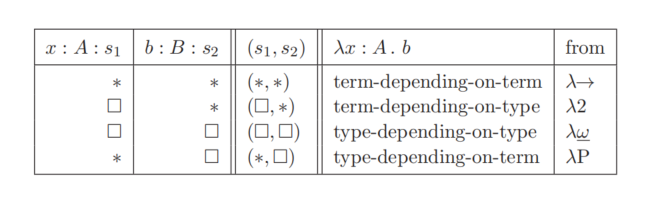
\includegraphics[width=0.93\linewidth]{"../imgs/6-1.png"}
		
	\section{$\lambda$-cube}
	\noindent
	对于$\lambda{\rightarrow}$基础上的三个扩展,彼此之间相互独立,可以被看作是扩展时的三个相互垂直的方向,给出坐标轴的三维系统:
		
		\noindent
		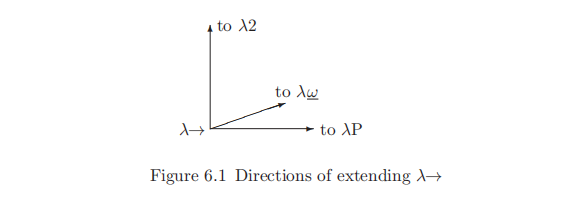
\includegraphics[width=0.93\linewidth]{"../imgs/6-2.png"}
		
		三个扩展共同组成了$\lambda{\rm C}$,而将$\lambda{\rightarrow}$与这三种扩展中的两个相组合而成的系统分别叫做$\lambda{\omega}$($\lambda{\rightarrow}+\lambda{2}+\lambda{\uline{\omega}}$),$\lambda{\rm P2}$和$\lambda{\rm P\uline{\omega}}$。
		
		所有的八个系统可以在一个立方体中定位,也即所谓的$\lambda{-{cube}}$或者巴伦德雷格立方体($Barendregt\ cube$):
		
		\noindent
		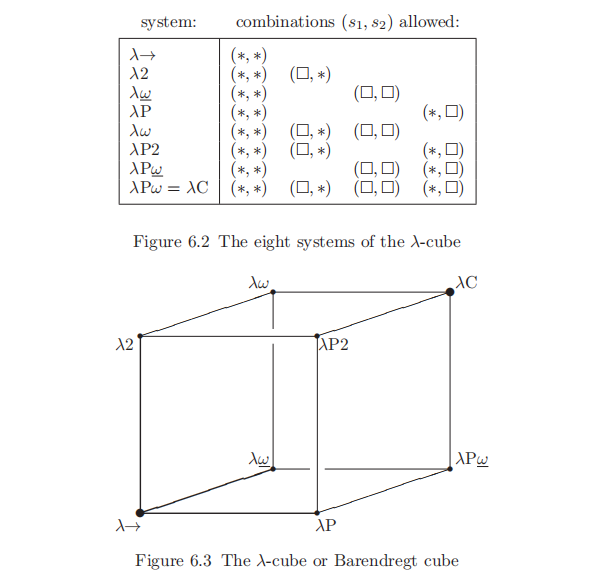
\includegraphics[width=0.93\linewidth]{"../imgs/6-3.png"}
		
		这八个不同的系统可以通过推导规则的唯一个集合来描述:
		
		\noindent
		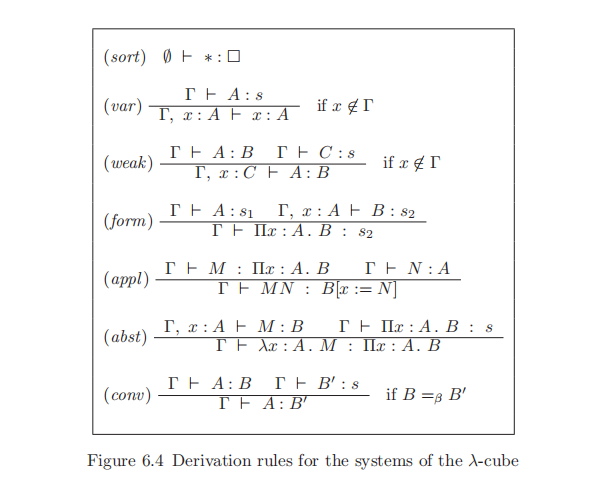
\includegraphics[width=0.93\linewidth]{"../imgs/6-4.png"}
		
		每一个系统都依赖于($s_1,s_2$)的组合,根据表 Figure 6.2 可得。以$\lambda{\uline{\omega}}$为例,只需要将$A\rightarrow B$看作是$\Pi x:A.B$的缩写,又因为$(s_1,s_2)\in\{(*,*),(\square,\square)\})$,所以再令$s_1=s_2=s$即可。
		
	\section{$\lambda{\rm C}$的性质}
	\noindent
	之前描述的大部分性质,$\lambda{\rm C}$依然保持,但措辞可能会有不同,对于某些直白的改变不再赘述。
	
		\begin{thm}($\lambda{\rm C}$的表达式,$\mathcal{E}$)
			
			$\lambda{\rm C}$的表达式的集合$\mathcal{E} = V|\square|*|(\mathcal{EE})|(\lambda V:\mathcal{E}.\mathcal{E})|(\Pi V:\mathcal{E}.\mathcal{E})$
		\end{thm}
	
		\begin{lemma}(自由变量引理)
			
			如果$\Gamma\vdash A:B$,则$FV(A),FV(B)\subseteq dom(\Gamma)$
		\end{lemma}
		
		\begin{lemma}(良构的上下文)
			
			如果存在$A$和$B$使得$\Gamma\vdash A:B$,则上下文$\Gamma$是良构的。
		\end{lemma}
	
		\begin{lemma}(压缩引理,Condensing Lemma)
			
			如果$\Gamma',x:A,\Gamma''\vdash B:C$且$x$不在$\Gamma'', B, C$中出现,则有$\Gamma', \Gamma''\vdash B:C$。
		\end{lemma}
	
		需要注意的是,压缩引理与 Lemma 2.10.5 不同:Lemma 2.10.5 中,所有多余声明可以一次性去掉,而新的引理中一次只能去除一个,因为$B,C$中的自由变量可能依赖于上下文中其它的变量。
		
		\begin{lemma}(替换引理)
			
			令$\Gamma',x:A,\Gamma''\vdash B:C$且$\Gamma'\vdash D:A$,则$\Gamma',\Gamma''\left[ x:=D\right]\vdash B
			\left[x:=D\right]:C\left[x:=D\right]$
		\end{lemma}
	
		\begin{lemma}(Subject Reduction)
			
			如果$\Gamma\vdash A:B$且$A\rightarrowtail_\beta A'$,则$\Gamma\vdash A':B$。
		\end{lemma}
	
		在第四章中提到过,($Subject Reduction$)引理可以直接证明,而($conv$)-规则需要显式给出,因为出现过的项不能在声明中(以相同含义)出现第二次,无法同时引出两个类型,而相同类型可以多次出现,推导出不同的项即可。
		
		\begin{thm}(Strong Normalisation Theorem / Termination Theorem)
			
			每一个合法的$M$都是 strongly normalising。
		\end{thm}
	
		\begin{thm}(良好定义和类型检查的可判定性)
			
			在$\lambda{C}$和它的子系统中,良好定义和类型检查都是可判定的。
		\end{thm}
	
		项查找在$\lambda{\rightarrow}$和$\lambda{\uline{\omega}}$中是可判定的,但是在剩余的系统中是不可判定的。
		
		尽管项查找在许多时候是不可判定的,但是计算机可以为定理证明提供大量的帮助,通过提供一些开放的目标,或者检查推导的过程是否符合规则。这样的程序被称为“证明助手(proof assistants)”,在帮助人们解决逻辑或者代数问题时越来越有用,它们同样被用于证明计算机程序的正确性,比如证明一个给定的计算机程序是否满足它的规范。
\end{document}
